% !TeX root = ../main.tex
% Add the above to each chapter to make compiling the PDF easier in some editors.

\chapter{Related Work}\label{chapter:related_work}

\section{Emission Inventories}
Emission inventories are a collection of emission data of pollutants or greenhouse gases (GHGs) released into the atmosphere over a specified period within a defined geographic area.
They serve as foundational tools for environmental management, policy formulation, and compliance with international agreements on climate change mitigation.
Typically, these inventories are constructed using bottom-up methodologies, where emissions are calculated at the most granular level, i.e. individual sources, and then aggregated to provide a comprehensive overview.

The bottom-up approach involves collecting detailed activity data for each emission source, such as fuel consumption rates, industrial production volumes, or agricultural practices.
Emission factors, representing the average emissions per unit of activity, are then multiplied with these data, resulting in an estimate of the total emissions of that source.
This method allows for a high degree of specificity and enables sectoral analysis, making identification of key emission contributors possible.

While emission inventories offer detailed estimates, they can be inaccurate due to incomplete data, outdated emission factors, and the exclusion of unknown or hidden emission sources.
These limitations highlight the need for top-down approaches, where atmospheric measurements are used to reconstruct emission sources, potentially identifying overlooked emitters [Bergamaschi et al., 2018].

% Emission inventories are essential tools for monitoring anthropogenic GHG emissions.
% They provide spatially and temporally resolved estimates of emissions based on activity data (e.g., fuel consumption, industrial processes) and emission factors.
% Inventories like the CAMS (Copernicus Atmosphere Monitoring Service) and TNO datasets provide detailed emission fields across Europe with varying spatial resolutions [CAMS 2020; TNO 2020].
% These inventories are typically used for bottom-up estimates, where emissions are computed by aggregating activity data from individual sectors, such as transportation, residential heating, and industry.


% Emission inventories are a estimation of emission fields
% They serve two main purposes \parencite{CAMS-REG-v4}.
% The first purpose is to 
% Questions:
% \begin{enumerate}
%     \item what are the purpose of emission inventories
%     \item what are Emission Inventories
%     \item How are Emission Inventories generated
%     \item what are the problems with bottom-up approaches for GHG emissions? 
%     \subitem may miss
%     \item what are typical approaches to top-down?
%     \item what are the challenges in top-down approaches?
% \end{enumerate}
% Then go over to Benjis work who has shown that 
% For this work, same assumptions as in Benjis work hold, i.e. background GHG emissions are ignored.

% Bottom-up approaches estimate emission fluxes by multiplying emission sources with their activity \parencite{BU-vs-TD} (also cite inventories).
% In contrast, top-down approaches start from measurements of GHG conecntrations and invert the transport of molecules to find the sources from which they emitted.
% One example for a measurement network is MUCCnet \parencite{MUCCnet}.
% Bottom-up approaches can miss emitters due to unknown datas whereas top-down approaches can be able to capture unknown emitters with measurements.
% Furthermore, 
% Bottom-up and top-down approaches show gaps in their esimtations which can largely be explained by temporal variability \parencite{BU-vs-TD}.

% There are essentially two approaches to estimating emissions.
% The first approach starts from the and is called bottom-up approach.
% The second approach starts from measurements and aims at inverting the atmospheric transport of molecules to determine the sources.

% \begin{enumerate}
%     \item 
% \end{enumerate}

\section{Atmospheric Inversion}
Top-down approaches formulate the emission estimation problem as an inverse problem, where GHG concentrations measured at ground-based or satellite stations are used to infer the underlying emission fields.
An example for a sensor network doing such measurements is the MUCCnet sensor network.
From these measurements, the emission field is reconstructed by applying inversion techniques. 

One such technique is Bayesian inversion.
Bayesian inversion updates prior knowledge about emissions using a likelihood function derived from measurement data [Rodgers, 2000; Ganesan et al., 2014].
However, these methods often rely heavily on accurate priors, which can introduce bias when prior information is incomplete or incorrect.
In urban areas, where emissions can vary greatly in space and time, such methods may struggle to provide accurate results without prior assumptions.

To overcome the limitations of Bayesian methods, recent studies have explored sparse reconstruction techniques.
These methods assume that emissions are spatially sparse (i.e., only a few large sources contribute significantly to the total emissions) and use optimization techniques to recover the emission field from a limited set of measurements.
Works by Benisch et al. (2020) and Turner et al. (2016) demonstrated that compressed sensing approaches can be effective for reconstructing urban GHG emissions, especially when combined with sparse priors or transforms, such as wavelets or discrete cosine transforms (DCT).

% How do top down approaches work?
% What is the inverse problem?
% Benji deonstrated use of compressed sensing.
% Formulate the problem formulation for this thesis here.
% Meaning, what are the constraints.
% Background GHG emissions.
% Assume linear forward model.

% This inverse problem can be solved using Bayesian inversion.
% Mention l2 norm reconstruction.

\section{Compressed Sensing}
Compressed Sensing (CS) is a mathematical framework that enables the recovery of sparse signals from a reduced number of measurements.
The fundamental assumption behind compressed sensing is that the signal of interest is either sparse or compressible in some domain, meaning that most of its components are zero or near-zero.
This property allows for the accurate reconstruction of signals even when the number of measurements is significantly smaller than the number of unknowns.

The standard compressed sensing formulation in the context of urban GHG emission estimation is represented as follows:
\begin{equation}
    y = A x + \epsilon
\end{equation}
where $y \in R$ represents the vector of measurements (e.g., atmospheric GHG concentrations), $A \in R^{m \times n}$ is the sensing matrix that models the relationship between the measurements and the emissions, $x \in R^n$ is the unknown signal (i.e., the emission field), and $\epsilon$ is the noise term, capturing errors or uncertainties in the measurement process.
The sensing matrix $A$ represent the atmospheric transport of molecules and is derived from atmospheric transport models, such as STILT.
Due to a lack of measurements, this problem is ill-posed.
In urban settings, where emissions are typically sparse originating from a few dominant sources such as industrial facilities or traffic hubs compressed sensing provides a natural framework for recovering the emission field from a limited set of observations.

There are many sparse reconstruction algorithms.
One of the most commonly used one is the Lasso algorithm, which solves the inverse problem by enforcing sparsity through L1-norm regularization.
Another prominent approach is Basis Pursuit (BP), which directly seeks the sparsest solution, and its variant, Basis Pursuit with Denoising (BPDN), which extends the model to handle noisy measurements.
These methods are crucial in emission estimation, where high-dimensional emission fields need to be recovered from a small number of measurements taken by atmospheric sensors.

The Lasso (Least Absolute Shrinkage and Selection Operator) algorithm is a widely used method in compressed sensing due to its ability to enforce sparsity in the solution.
It achieves this by solving the following optimization problem:
\begin{equation}
    \min{\left( \norm{Ax -y }_2^2 + \alpha\norm{x}_1 \right)}
\end{equation}

In this formulation, $\norm{Ax -y }_2^2$ is the least-squares term that measures the discrepancy between the observed measurements $y$ and the predicted measurements $Ax$, while $\norm{x}_1$ represents the L1-norm of the signal, promoting sparsity.
The parameter $\alpha$ controls the trade-off between the accuracy of the fit and the sparsity of the solution.
A larger $\alpha$ results in a sparser solution, whereas a smaller $\alpha$ allows for a closer fit to the observed data but may introduce non-zero components in $x$, leading to less sparsity.

% The Lasso algorithm is particularly suitable for GHG emission estimation because urban emission fields are often sparse, meaning that only a small fraction of locations contribute significantly to the total emissions.
% By minimizing the L1-norm, Lasso effectively drives many components of the emission field to zero, thus recovering the sparse structure of the emissions.
% However, the choice of $\lambda$ is crucial, as an excessively high value can result in an overly sparse solution that underestimates the true emissions, while a low value can lead to overfitting.

Basis Pursuit (BP) is another widely adopted algorithm for sparse reconstruction, particularly when the goal is to find the sparsest possible solution that satisfies the measurement constraints exactly.
Basis pursuit solves the following optimization problem:
\begin{equation}
    \min \norm{x}_1 \quad \text{subject to} \quad  Ax = y
\end{equation}

Here, the objective is to minimize the L1-norm of the signal, ensuring that the predicted measurements $A x$ match the observed measurements $y$ exactly.
In contrast to Lasso, basis pursuit does not include a regularization term and instead focuses solely on finding the sparsest solution that satisfies the measurement equation.

Basis pursuit is ideal when the measurement process is noiseless and the sensing matrix $A$ satisfies the Restricted Isometry Property (RIP), ensuring that different sparse signals remain distinguishable.
However, in real-world applications, such as atmospheric GHG monitoring, measurements are rarely noise-free, and enforcing $Ax = y$ strictly can lead to inaccurate reconstructions when noise is present.

To address the limitations of basis pursuit in noisy environments, Basis Pursuit with Denoising (BPDN) introduces a tolerance for noise in the measurement process.
BPDN modifies the original basis pursuit problem by allowing deviations from the exact measurement equation:
\begin{equation}
    \min \norm{x}_1 \quad \text{subject to} \quad  Ax -y \le \delta
\end{equation}

In this formulation, $\delta$ represents the allowable level of noise or error in the measurements.
The L1-norm is minimized to promote sparsity in the signal, while the L2-norm ensures that the predicted measurements are close to the observed measurements within a defined noise threshold.
The parameter $\delta$ allows BPDN to flexibly handle noisy data, making it more suitable for real-world scenarios, such as urban GHG emission estimation, where measurement noise is inevitable due to sensor inaccuracies and atmospheric variability.

Basis Pursuit with Denoising strikes a balance between sparsity and measurement accuracy, making it particularly useful when the sensing matrix $A$ does not fully satisfy RIP or when the measurement process involves significant noise.
By allowing for a controlled level of error, BPDN can recover the sparse emission field without being overly sensitive to noise, resulting in more robust solutions.

% What is compressed sensing?
% When does it work?
% For emission fields in cities with point sources, this works well as the emission field is sparse.

% Here, I should explain the general theory of compressed sensing.
% Compressed sensing makes assumptions about the signal and forward model.
% Generally, signals are assumed to be sparse in some basis.
% If the forward model then fulfills certain criteria, reconstruction can be gurantueed.
% Sparsity can be 

% [Citations mssing]
% The most basic algorithm to reconstruct a signal would be minimize the L0 norm of a signal.
% The L0 norm is defined as the number of all non-zeros elements of a vector.
% \begin{equation}
%     min L0 of  s.t. y = Ax
% \end{equation}
% This problem is NP-hard and thus not practical in real world applications.
% Instead, it can be shown that minimizing the L1 norm yields the same result as above under certain conditions.
% \begin{equation}
%     \min()
% \end{equation}
% This algorithm is known as basis pursuit (BP).

% Basis pursuit is a very powerful algorithm, but assumes that measurements are ideal, i.e. not noisy.
% Extensions of this algorithm exist that deal with noise.
% This extension is called basis pursuit denoising (BPDN)
% \begin{equation}
%     \min()
% \end{equation}
% BPDN thus assumes that the noise level is known.

% Furthermore, regularization teqhniues exist to also sovle comrpessed sensing problems, for instance the Lasso regularizer which assumes a Laplacian prior.
% \begin{equation}
%     Lasso
% \end{equation}
% It can be shown that BPDN is equivalent to the Lasso regularizer for a certain alpha.

% For compressed sensing, signals must be sparse in some basis.
% This can be done with overcomplete dictionaries, transforms, etc.
% Common way is wavelet transform or discrete cosine transform.

% Recent developments make use of generative models for low dimensional representations which can be interpreted as sparse maps.
% This samples can be generated and thus represented with only few dimensions.

% There are three main approaches to alleviate sparsity constraint.
% 1) transforms, such as Wavelet
% 2) only searching for unknown emissions and take esimtations as basis
% 3) Deep learning based approaches
\section{Generative Models for Compressed Sensing}
Compressed sensing traditionally relies on the assumption that the underlying signals are sparse in some basis.
However, this assumption may not hold in all applications.
For instance, in urban emissions scenarios, while large point sources are often known or can be well-estimated, diffuse or area sources result in emission fields that are less sparse.
This lack of sparsity challenges the effectiveness of conventional compressed sensing techniques, potentially leading to reconstruction failures.

Generative models offer a promising alternative by relaxing the strict sparsity constraint.
These models learn complex representations directly from data, circumventing the need for pre-specified sparse bases.
Recent advancements in fields such as medical imaging have successfully applied generative models to solve compressed sensing problems (cite). %\parencite{jalal2021robust}).

In this thesis, we focus on the pioneering work by Bora et al. (cite), framework that leverages generative models to improve upon classical compressed sensing techniques.
Their approach demonstrates that by using neural networks trained to model the distribution of the underlying data, the performance of compressed sensing can be significantly enhanced.

\subsection{Generative Models}

Bora et al.'s framework primarily involves generative adversarial network (GAN) type models, including Variational Autoencoders (VAEs) and Generative Adversarial Networks (GANs).
Both VAEs and GANs generate samples from lower-dimensional noise, transforming a latent variable $z \in \mathbb{R}^d$ into a data sample $x \in \mathbb{R}^n$ through a generator function $G: \mathbb{R}^d \to \mathbb{R}^n$.

\textbf{Variational Autoencoders (VAEs)} are probabilistic models that encode input data into a latent space and then decode it back to the original space.
They optimize a variational lower bound on the data likelihood, effectively learning a smooth latent space that captures the data distribution.

\textbf{Generative Adversarial Networks (GANs)} consist of two neural networks—the generator $G$ and the discriminator $D$—trained in a minimax game.
The generator tries to produce data that is indistinguishable from real data, while the discriminator attempts to differentiate between real and generated data.
GANs are known for generating high-quality samples but can be challenging to train due to instability in the adversarial objectives.

While GANs often show superior quality in sample generation across various domains, their training instability makes them less suitable for some applications.
Therefore, this thesis chooses VAEs as the appropriate type of generative model due to their stability and structured latent space.

Besides Bora et al. work there are many different approaches (cite the overview).
For example, work using score-based or diffusion models (cite) in the context of medical imaging (cite).
Additionally, normalizing flows (cite) also show promising reults (cite).
But since the goal of this thesis is not to compare individual ML based compressed sensing approaches, the focus lies on Bora et al. work.

\subsection{The Range of a Generator}

The \textbf{range of a generator} $G$ refers to the set of all possible outputs $G(z)$ as $z$ varies over the latent space $\mathbb{R}^d$.
This range represents the subset of the signal space $\mathbb{R}^n$ that the generative model can produce.
In the context of compressed sensing, the reconstruction is constrained to lie within this range, which underscores the importance of the generative model accurately capturing the true data distribution.

\subsection{Compressed Sensing Framework}

Bora et al.'s approach operates by integrating generative models into the compressed sensing reconstruction process.
Given a linear measurement model:
\begin{equation}
    y = A x + \epsilon
\end{equation}
where $A \in \mathbb{R}^{m \times n}$ is the sensing matrix, $x \in \mathbb{R}^n$ is the unknown signal (e.g., an emission field), $y \in \mathbb{R}^m$ represents the measurements, and $\epsilon$ denotes noise, the goal is to recover $x$ from $y$.

The key idea is to leverage a pretrained generative model $G$ as a prior for $x$.
In contrast to Bayesian inversion which heavily relies on a predefined prior, which can be a major limitation if the prior does not accurately reflect the true spatial distribution of emissions.
A generative model would avoid this by learning the prior directly from the data.
The reconstruction problem is formulated as an optimization over the latent space:

\begin{equation}
    \min_{z}{\left( \norm{A G(z) - y}_2^2 + \gls{gamma} R(z) \right)}
\end{equation}
Here, $R(z)$ is a regularization term that encourages desirable properties in the solution, and $\gls{gamma}$ controls the strength of the regularization.
For instance, in the case of $z$ being Gaussian distributed, the regularization $R(z) = \norm{z}_2^2$ is used, similar to Ridge regression.
The generative model $G$ represents the range of possible signals, and the optimization seeks the latent vector $z$ that, when passed through $G$, produces a signal that matches the measurements $y$ as closely as possible.

Since $G$ is differentiable with respect to $z$, gradient-based optimization methods can be employed to solve the problem.
The optimization seeks the latent vector $z^{\star}$ such that $G(z^{\star})$ best explains the measurements $y$.

\begin{figure}[h!]
    \centering
    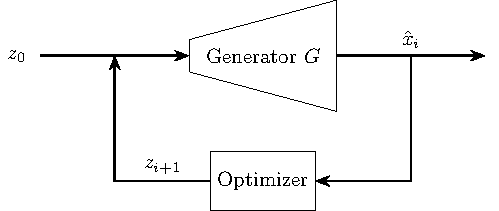
\includegraphics[width=0.75\textwidth]{figures/02_related_work/latent_variable_optimization/build/latent_variable_optimization.pdf}
    \caption{Bora et al paper}
    \label{fig:gen_solver}
\end{figure}

One limitation of Bora et al.'s method is that the reconstructed signal $G(z^{\star})$ is confined strictly to the range of $G$.
This constraint may be too restrictive if $G$ does not perfectly capture the true data distribution, leading to reconstruction errors.

To address this issue, Dhar et al. (cite) proposed an extension that allows for sparse deviations from the generator's output.
The modified optimization problem introduces an additional variable $s \in \mathbb{R}^n$ representing a sparse offset:

\begin{equation}
    \min_{z, s}{\left(\norm{s}_1 + \gls{lambda} \norm{A \left( G(z) + s \right) - y}_2^2 \right)}
    \label{eq:sparse_deviation}
\end{equation}
where $\norm{s}_1$ promotes sparsity in the offset $s$ and the parameter $\lambda$ balances the sparsity of $s$ with the fit to the measurements $y$.

The reconstructed signal is then given by $\hat{x} = G(z^\star) + s^\star$, where $z^\star$ and $s^\star$ are the solution to the optimization problem in Equation \ref{eq:sparse_deviation}.

This extension allows the reconstruction to deviate slightly from the generator's range, accommodating components of the signal not captured by $G$, while maintaining overall consistency with the measurements and promoting sparsity in the deviations.

% \section{Generative Models (old)}
% There are three main kinds of modern successful generative models in the context of sample generation.
% These models are not limited to image generation only.
% There are variational autoencoders, generative adverserial networks, and score based models.
% Both VAEs and GANs generate samples from lower dimensionional noise.
% Score based models generate samples by denoising previous samples, starting from noise.
% The noise and generated samples thus have same dimensions for score based models.
% Due to this, score based models are not directly applicable with the method from \parencite{CSUsingAI}.
% However, alternative approaches for score based models exist, which are not explored here.
% While GANs show higher quality generation for many different domains, GANs are difficult to train as the objectives can get very unstable.
% Therefore, for this thesis, VAE is chosen as the appropriate type of generative model

% \section{Generative Models for Compressed Sensing (old)}
% Compressed sensing typically relies on the assumption thatenerative model would avoid this by learning the prior directly from the data.
% This makes it adaptable to various scenarios without the need to manually define the prior.
% MENTION THIS HERE.
 the underlying signals are sparse in some basis.
% In urban emissions scenarios, Benji has shown that for many cities emissions are typically sparse, i.e. dominated by few large emitters.
% These large emitters are often covered as point sources in emission inventories.
% However, this thesis assumes that these large emitters can be well estimated and can therefore be assumed to be known.
% This changes the problem of atmospheric inversion.
% When looking at the diffuse or area sources, emission fields are less sparse and sparse reconstruction may fail.

% Generative models offer an alternative by relaxing the strict sparsity constraint.
% These models can learn complex representations directly from data and therefore circumvent the reliance on pre-specified sparse bases.
% Recent advancements in fields such as medical imaging have successfully applied generative models to solve compressed sensing problems (cite).
% For isntance, the score based method.

% For this thesis, we focus on the work by Bora et al. though.
% For instance, Bora et al. (2017) introduced a framework using generative models to reconstruct signals, leveraging deep learning to improve upon classical compressed sensing techniques.
% Their approach demonstrates that the performance of compressed sensing can be significantly enhanced by using neural networks trained to model the distribution of the underlying data.

% A typical generative model based compressed sensing approach operates as follows: given a linear measurement process $y = Ax + \epsilon$, where $A \in \mathbb{R}^{m \times n}$ is the sensing matrix, $x \in \mathbb{R}^n$ is the unknown emission field, and $\epsilon$ represents noise, the goal is to reconstruct $x$ from the measurements $y$.
% In this context, a generative model, $G: \mathbb{R}^d \to \mathbb{R}^n$, which maps a typically Gaussian distributed latent variable $z \in \mathbb{R}^d$ to the signal space, is used to solve the following optimization problem:
% \begin{equation}
%     \min_{z}{\left( \norm{A G(z) - y}_2^2 + \gls{gamma} R(z) \right)}
% \end{equation}

% Here, $R(z)$ is a regularization term that encourages desirable properties in the solution, and $\gls{gamma}$ controls the strength of the regularization.
% For instance, in the case of $z$ being Gaussian distributed, the regularization $R(z) = \norm{z}_2^2$ is used, similar to Ridge regression.
% The generative model $G$ represents the range of possible signals, and the optimization seeks the latent vector $z$ that, when passed through $G$, produces a signal that matches the measurements $y$ as closely as possible.
% In practice, as generative models $G$ are differentiable in $z$, this optimization problem is solved using numerical solvers with gradient descent as seen in Figure \ref{fig:gen_solver}.
% \begin{figure}[h!]
%     \centering
%     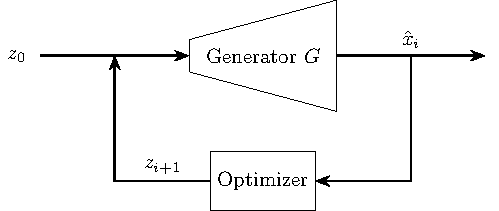
\includegraphics[width=0.75\textwidth]{figures/02_related_work/latent_variable_optimization/build/latent_variable_optimization.pdf}
%     \caption{Bora et al paper}
%     \label{fig:gen_solver}
% \end{figure}

% While this approach demonstrates promise, one significant limitation is that the reconstructed signal is constrained to lie within the range of the generator $G$.
% In other words, the reconstruction quality depends heavily on how well the generative model has learned the true distribution of the emission fields.
% To address this, subsequent work by Dhar et al. (2018) introduced methods that allow for sparse deviations from the generated signal, adding flexibility to the reconstruction.
% Their improved model solves the following optimization problem:
% \begin{equation}
%     \min_{z, s}{\left(\norm{s}_1 + \gls{lambda} \norm{A \left( G(z) + s \right) - y}_2^2 \right)}
%     \label{eq:sparse_deviation}
% \end{equation}
% The reconstructed signal is then $\hat{x} = G(z^\star) + s^\star$, where $z^\star$ and $s^\star$ are the solution to Equation \ref{eq:sparse_deviation}.

% As mentioned earlier, compressed sensing relies heavily on the signals being sparse in some basis.
% Zanger et al. have demonstrated that most cities are sparse enough for sparse reconstruction.
% Inventories like TNO split the emissions into area and point sources.
% The point sources are individual locations like power plants.
% These point sources are typically well known and make up a large portion of emissions.
% Once these are ignored, the emission fields are not as sparse anymore and sparse reconstruction does not work as well anymore.
% In this thesis, point sources are assumed to be well known and the primary target is reconstruction of area or diffuse sources.
% Luckily, generative models can be used for compressed sensing.
% This alleviates the constraint of sparsity for compressed sensing.

% Here I want to give an overview of generative models can be used for compressed sensing.
% I should use the review as reference and give a short summary.

% The field of medical imaging has made advancements in the inverse problems using deep learning.
% A review of different deep learning approaches for CS is given in \parencite{ReviewCSUsingAI}
% They mention Bora et al \parencite{CSUsingAI}.
% Their approach has the limitation that the reconstruction is constrained to the range of the generator.
% This, however, can improved by also taking into account other things: \parencite{SparseCSUsingAI}.

% Make a diagram of how the generative models are used.
% \begin{figure}[h!]
%     \centering
%     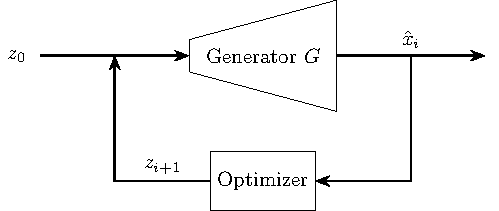
\includegraphics[width=0.75\textwidth]{figures/02_related_work/latent_variable_optimization/build/latent_variable_optimization.pdf}
%     \caption{Bora et al Paper}
% \end{figure}

% Assuming a linear forward model $y = Ax + \epsilon$ with $A \in \mathbb{R}^{m \times n}$
% Given is a generator $G: \mathbb{R}^d \to \mathbb{R}^n$ and the compressed sensing problem.
% Solve the following minimization problem:
% \begin{equation}
%     \min_{z}{\left( \norm{A G(z) - y}_2^2 + \gls{gamma} R(z) \right)}
% \end{equation}
% An improvements is made by to further consider sparse deviations from the generated emission fields:
% This equation is not quite right as it outsputs 2...
% \begin{equation}
%     \min_{z, s}{\left(\norm{s}_1 + \gls{lambda} \norm{A \left( G(z) + s \right) - y}_2^2 \right)}
% \end{equation}

% In contrast to Bayesian inversion which heavily relies on a predefined prior, which can be a major limitation if the prior does not accurately reflect the true spatial distribution of emissions.
% A generative model would avoid this by learning the prior directly from the data.
% This makes it adaptable to various scenarios without the need to manually define the prior.
% MENTION THIS HERE.

\section{Contributions}
In this work we make the following two assumptions:
\begin{enumerate}
    \item background emissions are known
    \item large emitters are accurately estimated
\end{enumerate}

The point of this work is not to investigate whether compressed sensing theory can be applied in the context of 
This has been investigated by prior work, like Benjis.
The point of this thesis is to investigate whether generative models can be applied.

Is the model able to generalize beyond the trianing data?
Is the model able to reconstruct emitters that are not covered in the emission inventories? 
What is a good dimension for the lower dimensional space?

Mention the rough constributions of this work:
\begin{enumerate}
    \item trained VAE for emission inventories of European cities
    \item demonstrated the applicability of generative models in the context of inverse models for top-down approaches
\end{enumerate}
